\addchapheadtotoc

\chapter{Introduction} \label{chapter:Introduction}
% Combustion has long been an effective means of energy conversion. Transportation systems, building heating and cooling, and power for electrical grids are just a few examples of its many applications. Over 82\% of energy produced on earth is produced through combustion~\cite{2021BpEnergy}. 
% At the same time, the explosive nature of the process may also result in its unwanted presence (e.g. rocket explosions, forest fires, house-fires, detonative combustion).
% Combustion is therefore a process that both can be used and must be managed. 
% Meanwhile the ongoing focus to reduce global emissions also imposes restraints on combustion researchers and scientists. Pollutants such as CO${}_2$, nitrous oxides, and soot have been shown to have a negative influence on our environment.
% So while the energy storage and release mechanisms that accompany combustion prove convenient for a lot of systems, they simultaneously presents a challenge for engineers and researchers.
% The need for improvement management of thermal loads, greater interconnected transport systems, development of heat-resistant materials, and an ongoing push to reduce global emissions must be met with an enhanced understanding of these physical systems.
% This enhanced understanding requires thorough understanding of the complex fluid dynamics, heat transfer, and chemistry that accompany combustion.
% Radiation is one of the most prominent physical processes that occurs during... 

\section{Background/Motivation}
The study of thermal radiation in combustion has not only theoretical interest but also great practical importance. Radiant emission from crown fires, for example, has been shown to be the dominant mode of heat transfer and may lead to significantly enhanced flame spread~\cite{Valendik2008EffectEnvironment}. Conditions for prevalent heat transfer through radiation are also present in combustion devices for useful energy conversion such as gas-turbine engines and steam boilers.
Many performance-critical applications operate at high temperatures for optimal thermal efficiency, often exceeding the melting points of the surrounding materials, which requires optimal design of thermal management systems such as thermal barrier coatings.
An understanding of thermal radiation is necessary to gauge its dynamic, non-linear, and non-local role in the listed combustion systems and others.

An understanding of radiant heat transfer in combustion can be difficult to achieve experimentally, however, due to the multitude of environmental variables like weather, prohibitively high temperatures that can break sensors and equipment, and the high number of independent variables in the problem. As such, computational tools have become a valuable resource in predicting flame properties under safe and controlled conditions. Modeling of combustion often employs computational fluid dynamics (CFD) combined with a model for the chemical kinetics of the chemical reaction network. Radiant heat transfer is simulated using a separate radiation model, which predicts the redistribution of thermal energy through electromagnetic wave/photon propagation. In such multi-physics simulations, computational resources may quickly become a limiting factor. For example, the application of the highest fidelity models (i.e., detailed chemical mechanism combined with Kolmogorov-scale cell sizes and line-by-line accurate non-gray radiation modeling) in a combined simulation is computationally prohibitive beyond laboratory-scale flames. Extensive research has been devoted to reducing the computational expense of physical modeling tools while maintaining the necessary degree of fidelity to achieve physically correct results.

This thesis will focus on improving the performance of radiation models in combustion systems. The highest fidelity radiation model, Monte Carlo Ray Tracing, where random rays are emitted and traced through the CFD geometry, is applied alongside enhancements inspired by the computer graphics community: Graphics Processing Units (GPUs) and Bounding volume hierarchy (BVH) data structures. Line-by-line accurate non-gray modeling is used to account for spectral influences within the medium, and various ray-tracing algorithms are proposed. 


% Thermal radiation in combustion systems has attracted increasing attention in recent years~\cite{Liu2020TheFlames}.
% During a combustion process, high temperature chemical products such as CO$_2$, H$_2$O, CO, and particulate soot will emit radiation strongly, resulting in a significant redistribution of energy throughout the reacting flow and into the surroundings~\cite{Modest2022ChapterSystems}. In gas-turbine combustors, for example, this can result in significant changes to combustion chemistry [statistic], flow patterns [another statistic], and the overall thermodynamic cycle efficiency.

% High temperature combustion product molecules CO$_2$, H$_2$O, CO, and particulate soot will emit radiation strongly, resulting in a significant redistribution of energy throughout the reacting flow and into the surroundings~\cite{Modest2022ChapterSystems}. 
% For one, the increasing efficiency requirements in aeronautical combustors have resulted in gas temperatures exceeding $2100^{\circ}$C, which is higher than the melting points of the enclosing systems~\cite{Lefebvre2010GasCombustion}, and results in significant radiative heat loads amounting to up to $30$\% of the total heat flux to the combustion chamber and downstream turbine stages~\cite{Lefebvre1984FlameChambers,Flamant2019OpportunitiesCoatings}.
% For example, aeronautical engines tend to be designed to operate at higher temperatures and pressures, in order to improve the overall thermal efficiency.
% %high temperatures of combustion products may lead to high degrees of radiative emission.
% Consequently, the higher radiative loads will redistribute thermal energy throughout the combustor, and result in higher temperatures and radiative flux in the surrounding casing, changes in chemistry dynamics such as flame extinction and pollutant emissions, and, thermodynamically, a net energy loss from the system which can no longer contribute to any desired work output.
% In another example, radiation from wildland fires contributes extensively to the widespread propagation and expansiveness of a flame, totaling between 10\% and 90\% of the total energy flux, depending on the flame type and intensity~\cite{Westerling2016IncreasingSpring,Valendik2008EffectEnvironment,Sacadura2005RadiativeScience}. 
% The emission from the fire is known to heat nearby combustible materials, dry them substantially, and accelerate flame propagation, which may expose nearby firemen to scorching radiative loads of up to 12 kW/m$^2$~\cite{Valendik2008EffectEnvironment}.

\section{Influences of radiation in combustion}
A brief summary of known influences of radiation in combustion systems is listed here, with a more detailed literature survey provided in Chapter~\ref{chapter:Importance}.
Previous research has highlighted recurring trends, as discussed in reviews from Modest and Haworth~\cite{Modest2016RadiativeSystems}, Coehlo~\cite{Coelho2018RadiativeSystems}, and Liu et al.~\cite{Liu2020TheFlames}. 
\begin{itemize}
    \item Radiation contributes thermal energy at the same order of magnitude as convection to the boundaries of many enclosed combustion systems such as aeronautical combustors~\cite{Berger2016OnLoads,Johnson2021AnalysisMethod}
    \item Radiation has significance in pollutant formations (e.g. NO${}_x$ and soot) and highly temperature-sensitive phenomena due to its redistribution of thermal energy~\cite{Ihme2008ModelingFormulation,Habibi2007TurbulenceFlames,Ren2017MonteChamber}
    \item Sooting (i.e. luminous) flames often have more pronounced thermal radiation characteristics~\cite{Modest2016RadiativeSystems}
\end{itemize}
Regarding modeling of radiation in combustion simulations:
\begin{itemize}
    \item Neglecting radiative emission often results in temperature overprediction~\cite{Gamil2020AssessmentChamber}
    \item Neglecting radiative absorption often results in temperature underprediction~\cite{Ren2017MonteChamber}
    \item Accounting for turbulence-radiation interaction (TRI) increases radiative emission and reduces temperatures~\cite{Coelho2018RadiativeSystems}
    \item Non-gray modeling of radiation can increase radiative re-absorption compared to gray modeling~\cite{Wu2021LimitationsFires}
\end{itemize}


%Thermal radiation is often the most dominant form of heat transfer that accompanies many combustion systems. The high temperatures from the rapid energy release combined with heavily radiating combustion products result in a 

%Therefore, 
Misrepresentation of radiation in combustion modeling can lead to significant errors in the prediction of flame properties. These errors may present themselves, for example, in $200$~K differences of peak flame temperature in gas-turbines~\cite{Gamil2020AssessmentChamber}, $50$\% under-predictions of heat loss from a piston engine~\cite{Modest2016RadiativeSystems}, or $90$\% underpredictions of heat transfer from forest fires~\cite{Valendik2008EffectEnvironment}.
Therefore, comprehensive models of combustion phenomena should include the modeling of radiation to some degree.


% The modeling procedure of radiation in a participating medium; however, is complex and computationally expensive, as emission and absorption between every point within the fluid system must be accounted for. Consequently, despite its significant role, radiation is often accounted for using simplified models such as “optically thin” and “gray” models, or even neglected entirely, which may provide misleading and/or incomplete information pertaining the contribution of radiation~\cite{Liu2020TheFlames,Modest2016RadiativeSystems}. 
% The objective in this thesis is to develop faster radiation modeling approaches that can accurately account for its non-linear, non-local, and coupled influences to combustion. 

%\section{Influence of radiation from combustion processes}

%Oftentimes, radiation can present a damaging effect to surrounding objects.





%These influences drive scientists and engineers to produce faster and more accurate radiation models to couple to their combustion simulations.


% Many computational models have been proposed for radiation, oftentimes accompanying Computational Fluid Dynamics (CFD) solutions to model the fluid dynamics and chemistry. 
% The most accurate approach, Monte Carlo Ray Tracing (MCRT), requires a significant amount of computational resources. As a result, scientists and engineers have historically resorted to lower-fidelity radiation models at the cost of increased uncertainty.
% Over time; however, new implementations have emerged accelerating MCRT, largely driven by enhancements in computational hardware and software. 
% Scientists and engineers must continuously adapt their models to these new approaches in order to maintain the best available understanding of the influences of radiation in their studies. 




% Conversely, thermal radiation from combustion also provides meaningful contribution, oftentimes in a ways that are apparent in day to day life.
% The origins of the human usage of fire are believed to result from the radiative warmth that fire provides~\cite{Scott2018WhenDiscover,Baird2015WhenMe}.



% Thermal radiation plays an integral role in the recent advancements of combustion technologies.




% In its most ideal form, radiative emission energy takes the form of eq. \ref{eq:RadEnergy}.
% \begin{equation}
%     E_{rad}=\epsilon{}\sigma{}T^4
%     \label{eq:RadEnergy}
% \end{equation}
% Where E$_{rad}$ is the radiative emissive power in W/m$^3$, $\epsilon{}$ is the dimensionless emissivity (or emittance), $\sigma{}$ is the Stefan-Boltzmann constant in W/m$^2$K$^4$, and T is the temperature in Kelvin. 
% The fourth power relationship of emissive power with temperature represents a significant reason why radiation is often more prominent in combustion, where temperatures can reach upwards of $2000$ K~\cite{Modest2016RadiativeSystems}.
% The high heat fluxes can influence becomes important for pollutant formation, flame speeds, and threshold phenomena (near-limits)~\cite{Modest2016RadiativeSystems,Coelho2018RadiativeSystems,Liu2020TheFlames}. Including radiation can have an effect on the fluid dynamics, turbulence, boundaries, and mixture properties of a combustion simulation.

% Many turbulent flows are modeled using Reynolds-Averaged Navier-Stokes (RANS) and Large Eddy Simulations (LES), both of which rely on the averaging of the governing equations of combustion. This results in the need for models describing the unresolved fluctuations of radiative properties. The influence of unresolved scales on radiation is known as turbulence-radiation interaction (TRI). Emission-TRI and absorption-TRI are two radiative phenomena which can complicate radiation modeling, and have been extensively studied.


\section{Modeling challenge and approach}
%In attempt to maximize accuracy at the limitations of present resources, 
A number of models and solvers for the radiative transfer equation (RTE) have been introduced to model thermal radiation while minimizing computational burden.
Of those, many rely on complex mathematical assumptions and simplifications, such as the P-N method~\cite{Modest2008EllipticGeometries}, which can be difficult to derive and implement~\cite{Ge2015ImplementationOpenfoam}. 


The Monte Carlo Ray Tracing (MCRT) method stands out as the most accurate, robust, and conceptually simple of the available models~\cite{Tesse2002RadiativeApproach,Modest2013RadiativeTransfer,Coelho2018RadiativeSystems}, and is regarded by many to be the best radiation solver as computational power increases~\cite{Howell2010ThermalTransfer}.
In MCRT, random rays are initialized and traced from their source computational cell to other cells in the domain to stochastically approximate the transport of radiation throughout the geometry.
The resulting process can be intuitively thought of as the tracing of `photon packets' traveling through the domain.
As a result of this approach, MCRT can account for many of the same effects that electromagnetic rays undergo during their travel.

Although MCRT is often considered the most accurate, it has also been viewed traditionally as the most computationally expensive.
This additional cost results from the stochastic nature of MCRT. A large sample size of rays must be emitted and traced to obtain a statistically meaningful solution. 
Too few rays may result in excessive noise, while too many require a longer simulation runtime. In most situations, the ray-tracing procedure, in particular, is a bottleneck~\cite{Galtier2013IntegralAlgorithms}, as shown in Fig. \ref{fig:Sample_Profiling}, which presents the runtime profiling for a decoupled gray simulation of radiation in a backward-facing step combustor.
The limitations imposed by this bottleneck significantly inhibit the use of MCRT in combustion simulations. So far, the MCRT methods are mostly employed in decoupled form~\cite{Modest2022ChapterMedia} where single timestep is used for analysis. 

% Recently, much effort has been put into making the computation more manageable while maintaining the benefits MCRT in coupled combustion simulations~\cite{Liu2020TheFlames,Tesse2002RadiativeApproach,Zeeb2001AnGeometries,Modest2003BackwardTransfer,Howell2010ThermalTransfer}.
% THIS IS THE PLACE WHERE I WILL ADD YOUR OWN RESULTS WITH A FIGURE AS A MOTIVATION: PROFILING ANALYSIS OF A XXX SHOWS THAT RAY TRACING TAKES XXX PERCENTAGE OF THE RUNTIME AND IS THE BOTTLENECK OF THE MCRT METHOD. 
\begin{figure}
\centering
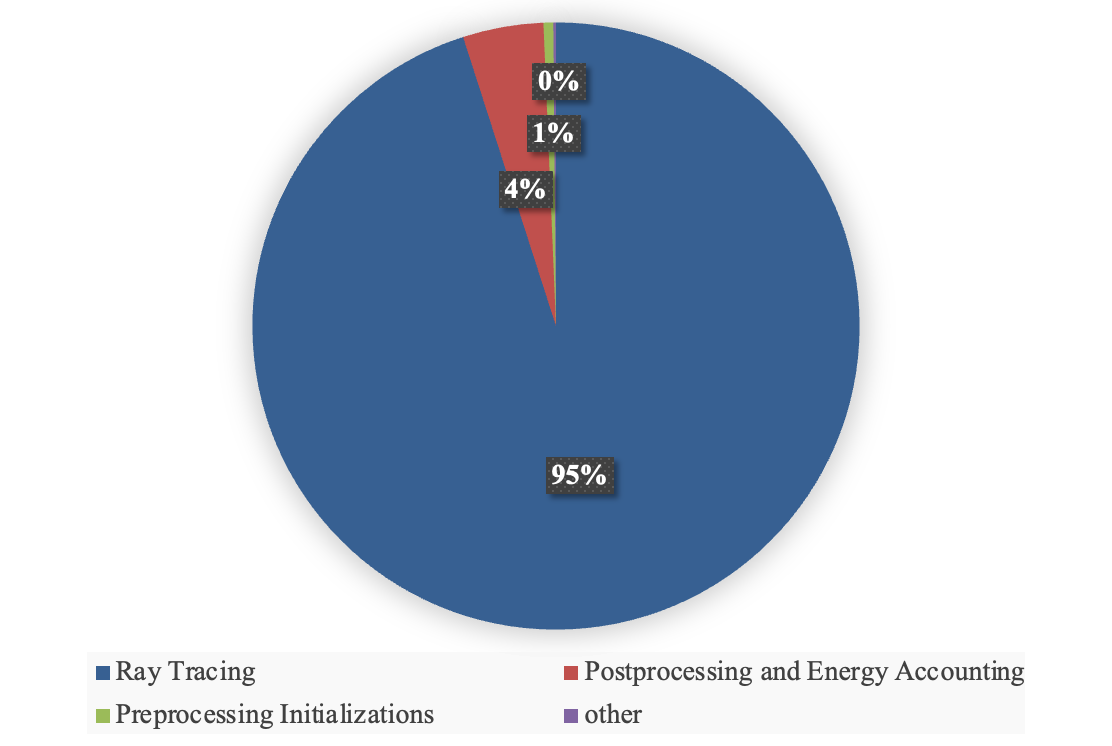
\includegraphics[width=0.8\linewidth]{figures/ch1/BFS_profiling.png}
\caption{Run-time breakdown of a Monte Carlo Ray Tracing radiative heat transfer simulation on a backward-facing step combustor (see section~\ref{section:BFS}).}
\label{fig:Sample_Profiling}
\end{figure}


Recently, Graphics Processing Units (GPUs) have demonstrated a significant potential to accelerate the Monte Carlo ray tracing process~\cite{Howell2021TheTransfer,Humphrey2015ATracing} by up to three orders of magnitude~\cite{Silvestri2019ASimulation}. Speedups at this level would significantly improve the applicability of MCRT in radiation modeling. 
Meanwhile, programming models such as Kokkos, which enable the use of an interchangeable parallel back-end, allow for easier implementation and code portability on CPUs or GPUs without any changes in the coding syntax~\cite{Trott_Kokkos3_2022}.


In this thesis, we implement an accelerated implementation of MCRT that is coupled with the open-sourced CFD platform \verb|OpenFOAM|~\cite{Weller1998ATechniques}.
This implementation relies on the Kokkos programming model for parallel computing on high performance computers~\cite{Trott2021KokkosEra}.
% Graphics Processing Units (GPUs) have been shown to dramatically accelerate the ray-tracing procedure, a process has been done very few times, but has shown significant speedups~\cite{Silvestri2019ASimulation,Humphrey2016RadiativeRefinement,Heymann2012GPU-basedAGN}. 
Also, the solver is implemented to utilize distributed-memory computing platforms through the use of the Message Passing Interface (MPI).
And finally, as an alternative to a standard ray tracing procedure, a geometric search library named ArborX~\cite{Lebrun-Grandie2019ArborX:Library} is introduced to implement a bounding-volume hierarchy data structure with backward Monte Carlo ray tracing (see section~\ref{section:ModelForThisStudy}).
% The BVH has shown great efficiency boosts for surface-to-surface ray tracing in the field of computer graphics~\cite{Meister2021ATracing}.
The present thesis will demonstrate how these changes can be used to bring speedup to the ray tracing procedure for thermal radiation in participating media without sacrificing accuracy.
% whether the efficient data structure can bring further speedup to the ray tracing procedure for participating media for thermal radiation.

\section{Organization}
In Chapter \ref{chapter:Importance}, we present a background on the fundamentals of thermal radiation and its importance in combustion. 
Then, in Chapter \ref{chapter:Modeling}, various Monte Carlo-based methods of solving the RTE are presented, including an overview of the present MCRT approaches, the supplemental libraries used, and a description of the solvers' coupling to \verb|OpenFOAM|. 
Chapter~\ref{chapter:Example} provides a verification of the solver in a plane-parallel medium and a demonstration of its performance using a backward-facing step combustor, a direct numerical simulation of a small turbulent pool fire, and a transient pool fire. Observations are made regarding the influence of radiation and computational speedup for each configuration.
Finally, conclusions and future work are discussed in Chapter~\ref{chapter:conclusion}.